% HeroQuest manual, using the Sol Negro manual's A4 visual style.
% pdflatex -jobname=manual-es "\def\manlang{es}% HeroQuest manual, using the Sol Negro manual's A4 visual style.
% pdflatex -jobname=manual-es "\def\manlang{es}% HeroQuest manual, using the Sol Negro manual's A4 visual style.
% pdflatex -jobname=manual-es "\def\manlang{es}% HeroQuest manual, using the Sol Negro manual's A4 visual style.
% pdflatex -jobname=manual-es "\def\manlang{es}\input{manual}"
\documentclass[a4paper,11pt]{article}
\providecommand{\manlang}{es}
\usepackage[utf8]{inputenc}
\usepackage[T1]{fontenc}
\usepackage{helvet}
\renewcommand{\familydefault}{\sfdefault}
\input{meta}
\input{lang-\manlang}
\usepackage[margin=2.2cm,top=2.4cm,bottom=2.4cm]{geometry}
\usepackage{graphicx,xcolor,booktabs,tabularx,array,float,caption,fancyhdr,eso-pic,parskip,microtype}
\usepackage[hidelinks,pdftitle={HeroQuest \tPlatform{} -- \tManual{} v\versionjuego},pdfauthor={DiHalt}]{hyperref}
\graphicspath{{images/}{img/}}
\definecolor{accent}{RGB}{\accentRGB}
\definecolor{sangre}{RGB}{190,50,35}
\definecolor{pergamino}{RGB}{246,239,226}
\definecolor{ink}{RGB}{8,8,20}
\captionsetup{font=small,labelfont=bf}
\setlength{\parindent}{0pt}
\setlength{\headheight}{14pt}
\setcounter{secnumdepth}{2}
\setcounter{tocdepth}{2}
\setlength{\emergencystretch}{2em}
\raggedbottom
\pagestyle{fancy}\fancyhf{}
\fancyhead[L]{\small\textcolor{accent}{\textbf{HEROQUEST}} \tPlatform}
\fancyhead[R]{\small\tManual}
\fancyfoot[C]{\small\thepage}
\renewcommand{\headrulewidth}{0.4pt}
\newcommand{\chapter}[1]{\section{\textcolor{accent}{#1}}}
\newcommand{\key}[1]{{\fboxsep=2.5pt\fbox{\textbf{\strut #1}}}}
\newcommand{\pant}[1]{\textbf{#1}}
\newcommand{\pantalla}[3][0.78]{\begin{figure}[!htbp]\centering\includegraphics[width=#1\linewidth]{#2}\caption{#3}\end{figure}}
\newcommand{\dospantallas}[3]{\begin{figure}[!htbp]\centering\includegraphics[width=0.485\linewidth]{#1}\hfill\includegraphics[width=0.485\linewidth]{#2}\caption{#3}\end{figure}}
\newcommand{\aviso}[2]{\par\medskip\noindent\fcolorbox{accent}{pergamino}{\parbox{\dimexpr\linewidth-2\fboxsep-2\fboxrule\relax}{\textbf{\color{accent}#1}\par\smallskip #2}}\par\medskip}
\newcommand{\ficha}[4]{\par\medskip\noindent\begin{minipage}[t]{0.20\linewidth}\vspace{0pt}\centering\includegraphics[width=0.70\linewidth]{#1}\end{minipage}\hfill\begin{minipage}[t]{0.77\linewidth}\vspace{0pt}{\large\bfseries\color{accent}#2}\par\smallskip{\small #3}\par\smallskip #4\end{minipage}\par\medskip}
\newcommand{\aventura}[2]{\subsection*{\color{accent}#1.\ #2}\addcontentsline{toc}{subsection}{#1.\ #2}}
\newcommand{\objetivo}[1]{\par\smallskip\textbf{\tObjective} #1\par}
\newcommand{\consejos}[1]{\par\smallskip\textbf{\tTips} #1\par}
\newcolumntype{L}{>{\raggedright\arraybackslash}X}
\begin{document}
\hypersetup{pageanchor=false}
% Full-page cover, as in the Sol Negro reference.
\thispagestyle{empty}
% Frame the original landscape artwork at a smaller scale: the complete
% painted HEROQUEST title fits across the page, above the manual details.
\AddToShipoutPictureBG*{%
\put(0,0){\color{ink}\rule{\paperwidth}{\paperheight}}%
\put(0.5\paperwidth,\paperheight){\makebox(0,0)[t]{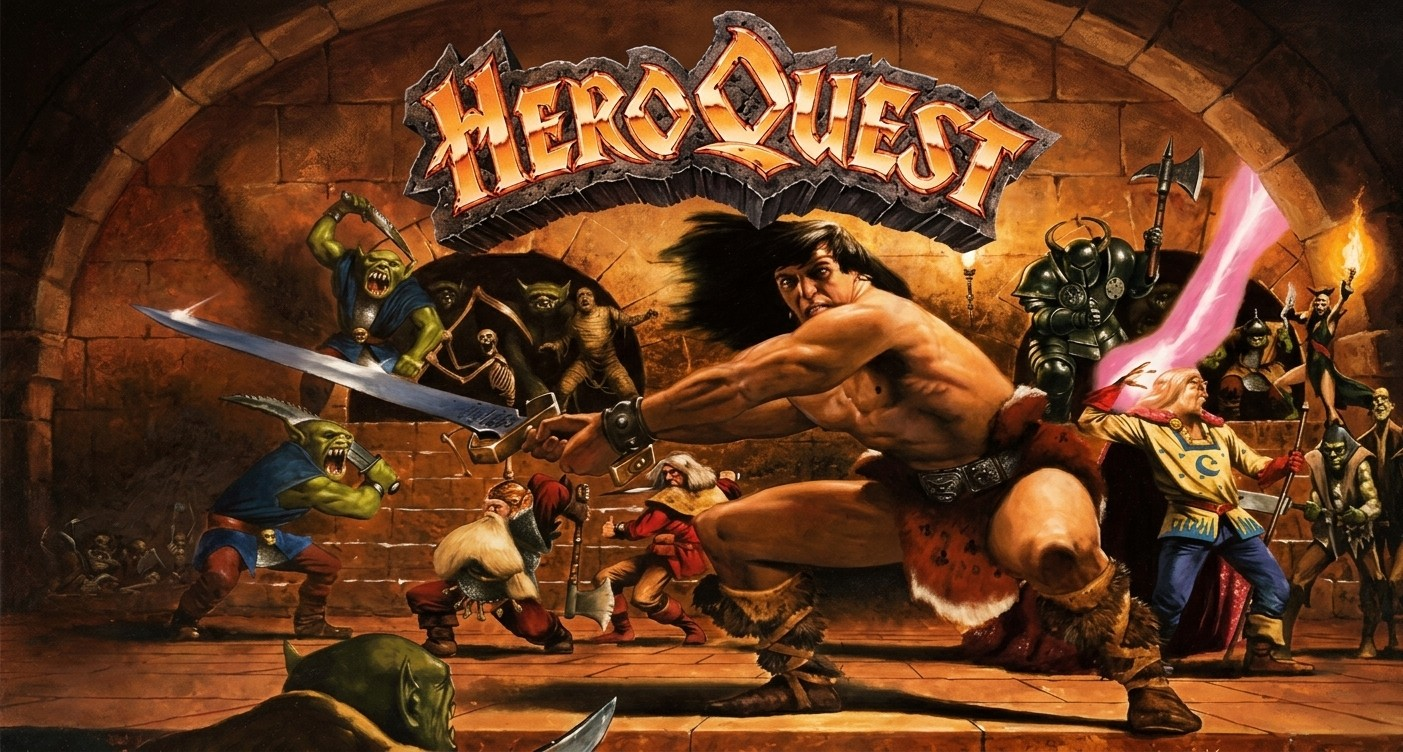
\includegraphics[width=1.6\paperwidth]{images/portada.jpg}}}%
\put(0.045\paperwidth,0.06\paperheight){
\includegraphics[width=0.30\paperwidth]{img/msx-logo.png}}}
\mbox{}\vfill
\begin{flushright}
\colorbox{ink}{\parbox{0.62\textwidth}{\raggedleft\color{white}\vspace{3pt}{\Huge\bfseries HEROQUEST}\\[6pt]{\Large\bfseries\tUserManual}\\[3pt]{\large\tPlatform{} \textperiodcentered{} \tVersion{} \versionjuego}\\[4pt]{\small\tCoverLine}\vspace{4pt}}}
\end{flushright}
\newpage
\thispagestyle{empty}
\begin{center}
\vspace*{1.2cm}
{\fontsize{34}{38}\selectfont\bfseries\textcolor{accent}{HEROQUEST}}\\[6pt]
{\Large\tPlatform}\\[1cm]

\includegraphics[height=2.2cm]{img/msx-logo.png}\\[1cm]
\tOriginal: \textbf{\originalPublisher}, \originalYear.\\[3pt]
\tPort: \textbf{\portAuthor}, \portYear.\\[3pt]
\tVersion{} \versionjuego\\[1cm]
\includegraphics[width=0.92\linewidth]{img/montage-\manlang.png}
\end{center}
\vfill
{\small\tHomage}
\newpage
\hypersetup{pageanchor=true}
\tableofcontents
\clearpage
\input{content-\manlang}
\clearpage
\input{credits-\manlang}
\input{label-\manlang}
\end{document}
"
\documentclass[a4paper,11pt]{article}
\providecommand{\manlang}{es}
\usepackage[utf8]{inputenc}
\usepackage[T1]{fontenc}
\usepackage{helvet}
\renewcommand{\familydefault}{\sfdefault}
% HeroQuest facts, shared by both editions.
\newcommand{\gameTitle}{HeroQuest}
\newcommand{\versionjuego}{1.0}
\newcommand{\originalPublisher}{Gremlin Graphics}
\newcommand{\originalYear}{1991}
\newcommand{\portAuthor}{DiHalt}
\newcommand{\portYear}{2026}
\newcommand{\accentRGB}{190,50,35}

\input{lang-\manlang}
\usepackage[margin=2.2cm,top=2.4cm,bottom=2.4cm]{geometry}
\usepackage{graphicx,xcolor,booktabs,tabularx,array,float,caption,fancyhdr,eso-pic,parskip,microtype}
\usepackage[hidelinks,pdftitle={HeroQuest \tPlatform{} -- \tManual{} v\versionjuego},pdfauthor={DiHalt}]{hyperref}
\graphicspath{{images/}{img/}}
\definecolor{accent}{RGB}{\accentRGB}
\definecolor{sangre}{RGB}{190,50,35}
\definecolor{pergamino}{RGB}{246,239,226}
\definecolor{ink}{RGB}{8,8,20}
\captionsetup{font=small,labelfont=bf}
\setlength{\parindent}{0pt}
\setlength{\headheight}{14pt}
\setcounter{secnumdepth}{2}
\setcounter{tocdepth}{2}
\setlength{\emergencystretch}{2em}
\raggedbottom
\pagestyle{fancy}\fancyhf{}
\fancyhead[L]{\small\textcolor{accent}{\textbf{HEROQUEST}} \tPlatform}
\fancyhead[R]{\small\tManual}
\fancyfoot[C]{\small\thepage}
\renewcommand{\headrulewidth}{0.4pt}
\newcommand{\chapter}[1]{\section{\textcolor{accent}{#1}}}
\newcommand{\key}[1]{{\fboxsep=2.5pt\fbox{\textbf{\strut #1}}}}
\newcommand{\pant}[1]{\textbf{#1}}
\newcommand{\pantalla}[3][0.78]{\begin{figure}[!htbp]\centering\includegraphics[width=#1\linewidth]{#2}\caption{#3}\end{figure}}
\newcommand{\dospantallas}[3]{\begin{figure}[!htbp]\centering\includegraphics[width=0.485\linewidth]{#1}\hfill\includegraphics[width=0.485\linewidth]{#2}\caption{#3}\end{figure}}
\newcommand{\aviso}[2]{\par\medskip\noindent\fcolorbox{accent}{pergamino}{\parbox{\dimexpr\linewidth-2\fboxsep-2\fboxrule\relax}{\textbf{\color{accent}#1}\par\smallskip #2}}\par\medskip}
\newcommand{\ficha}[4]{\par\medskip\noindent\begin{minipage}[t]{0.20\linewidth}\vspace{0pt}\centering\includegraphics[width=0.70\linewidth]{#1}\end{minipage}\hfill\begin{minipage}[t]{0.77\linewidth}\vspace{0pt}{\large\bfseries\color{accent}#2}\par\smallskip{\small #3}\par\smallskip #4\end{minipage}\par\medskip}
\newcommand{\aventura}[2]{\subsection*{\color{accent}#1.\ #2}\addcontentsline{toc}{subsection}{#1.\ #2}}
\newcommand{\objetivo}[1]{\par\smallskip\textbf{\tObjective} #1\par}
\newcommand{\consejos}[1]{\par\smallskip\textbf{\tTips} #1\par}
\newcolumntype{L}{>{\raggedright\arraybackslash}X}
\begin{document}
\hypersetup{pageanchor=false}
% Full-page cover, as in the Sol Negro reference.
\thispagestyle{empty}
% Frame the original landscape artwork at a smaller scale: the complete
% painted HEROQUEST title fits across the page, above the manual details.
\AddToShipoutPictureBG*{%
\put(0,0){\color{ink}\rule{\paperwidth}{\paperheight}}%
\put(0.5\paperwidth,\paperheight){\makebox(0,0)[t]{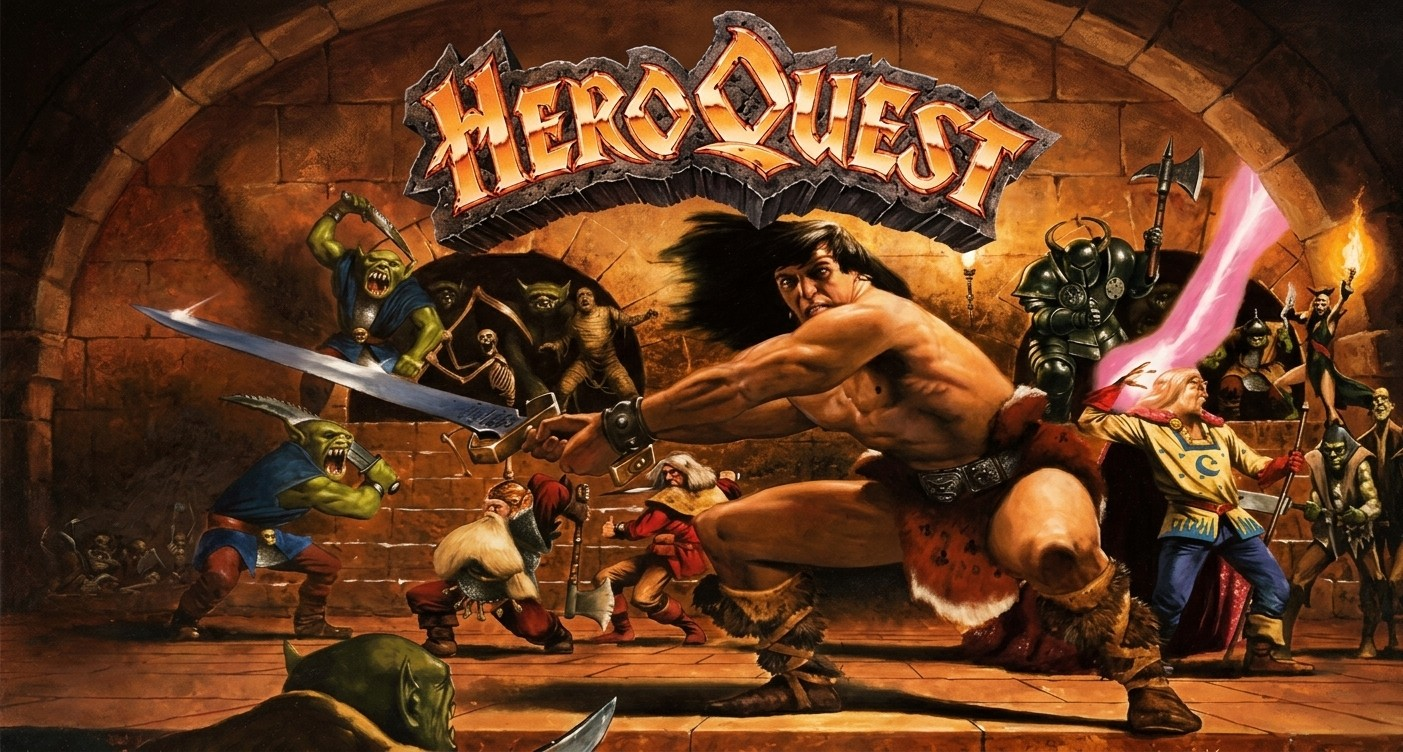
\includegraphics[width=1.6\paperwidth]{images/portada.jpg}}}%
\put(0.045\paperwidth,0.06\paperheight){
\includegraphics[width=0.30\paperwidth]{img/msx-logo.png}}}
\mbox{}\vfill
\begin{flushright}
\colorbox{ink}{\parbox{0.62\textwidth}{\raggedleft\color{white}\vspace{3pt}{\Huge\bfseries HEROQUEST}\\[6pt]{\Large\bfseries\tUserManual}\\[3pt]{\large\tPlatform{} \textperiodcentered{} \tVersion{} \versionjuego}\\[4pt]{\small\tCoverLine}\vspace{4pt}}}
\end{flushright}
\newpage
\thispagestyle{empty}
\begin{center}
\vspace*{1.2cm}
{\fontsize{34}{38}\selectfont\bfseries\textcolor{accent}{HEROQUEST}}\\[6pt]
{\Large\tPlatform}\\[1cm]

\includegraphics[height=2.2cm]{img/msx-logo.png}\\[1cm]
\tOriginal: \textbf{\originalPublisher}, \originalYear.\\[3pt]
\tPort: \textbf{\portAuthor}, \portYear.\\[3pt]
\tVersion{} \versionjuego\\[1cm]
\includegraphics[width=0.92\linewidth]{img/montage-\manlang.png}
\end{center}
\vfill
{\small\tHomage}
\newpage
\hypersetup{pageanchor=true}
\tableofcontents
\clearpage
\input{content-\manlang}
\clearpage
\input{credits-\manlang}
\input{label-\manlang}
\end{document}
"
\documentclass[a4paper,11pt]{article}
\providecommand{\manlang}{es}
\usepackage[utf8]{inputenc}
\usepackage[T1]{fontenc}
\usepackage{helvet}
\renewcommand{\familydefault}{\sfdefault}
% HeroQuest facts, shared by both editions.
\newcommand{\gameTitle}{HeroQuest}
\newcommand{\versionjuego}{1.0}
\newcommand{\originalPublisher}{Gremlin Graphics}
\newcommand{\originalYear}{1991}
\newcommand{\portAuthor}{DiHalt}
\newcommand{\portYear}{2026}
\newcommand{\accentRGB}{190,50,35}

\input{lang-\manlang}
\usepackage[margin=2.2cm,top=2.4cm,bottom=2.4cm]{geometry}
\usepackage{graphicx,xcolor,booktabs,tabularx,array,float,caption,fancyhdr,eso-pic,parskip,microtype}
\usepackage[hidelinks,pdftitle={HeroQuest \tPlatform{} -- \tManual{} v\versionjuego},pdfauthor={DiHalt}]{hyperref}
\graphicspath{{images/}{img/}}
\definecolor{accent}{RGB}{\accentRGB}
\definecolor{sangre}{RGB}{190,50,35}
\definecolor{pergamino}{RGB}{246,239,226}
\definecolor{ink}{RGB}{8,8,20}
\captionsetup{font=small,labelfont=bf}
\setlength{\parindent}{0pt}
\setlength{\headheight}{14pt}
\setcounter{secnumdepth}{2}
\setcounter{tocdepth}{2}
\setlength{\emergencystretch}{2em}
\raggedbottom
\pagestyle{fancy}\fancyhf{}
\fancyhead[L]{\small\textcolor{accent}{\textbf{HEROQUEST}} \tPlatform}
\fancyhead[R]{\small\tManual}
\fancyfoot[C]{\small\thepage}
\renewcommand{\headrulewidth}{0.4pt}
\newcommand{\chapter}[1]{\section{\textcolor{accent}{#1}}}
\newcommand{\key}[1]{{\fboxsep=2.5pt\fbox{\textbf{\strut #1}}}}
\newcommand{\pant}[1]{\textbf{#1}}
\newcommand{\pantalla}[3][0.78]{\begin{figure}[!htbp]\centering\includegraphics[width=#1\linewidth]{#2}\caption{#3}\end{figure}}
\newcommand{\dospantallas}[3]{\begin{figure}[!htbp]\centering\includegraphics[width=0.485\linewidth]{#1}\hfill\includegraphics[width=0.485\linewidth]{#2}\caption{#3}\end{figure}}
\newcommand{\aviso}[2]{\par\medskip\noindent\fcolorbox{accent}{pergamino}{\parbox{\dimexpr\linewidth-2\fboxsep-2\fboxrule\relax}{\textbf{\color{accent}#1}\par\smallskip #2}}\par\medskip}
\newcommand{\ficha}[4]{\par\medskip\noindent\begin{minipage}[t]{0.20\linewidth}\vspace{0pt}\centering\includegraphics[width=0.70\linewidth]{#1}\end{minipage}\hfill\begin{minipage}[t]{0.77\linewidth}\vspace{0pt}{\large\bfseries\color{accent}#2}\par\smallskip{\small #3}\par\smallskip #4\end{minipage}\par\medskip}
\newcommand{\aventura}[2]{\subsection*{\color{accent}#1.\ #2}\addcontentsline{toc}{subsection}{#1.\ #2}}
\newcommand{\objetivo}[1]{\par\smallskip\textbf{\tObjective} #1\par}
\newcommand{\consejos}[1]{\par\smallskip\textbf{\tTips} #1\par}
\newcolumntype{L}{>{\raggedright\arraybackslash}X}
\begin{document}
\hypersetup{pageanchor=false}
% Full-page cover, as in the Sol Negro reference.
\thispagestyle{empty}
% Frame the original landscape artwork at a smaller scale: the complete
% painted HEROQUEST title fits across the page, above the manual details.
\AddToShipoutPictureBG*{%
\put(0,0){\color{ink}\rule{\paperwidth}{\paperheight}}%
\put(0.5\paperwidth,\paperheight){\makebox(0,0)[t]{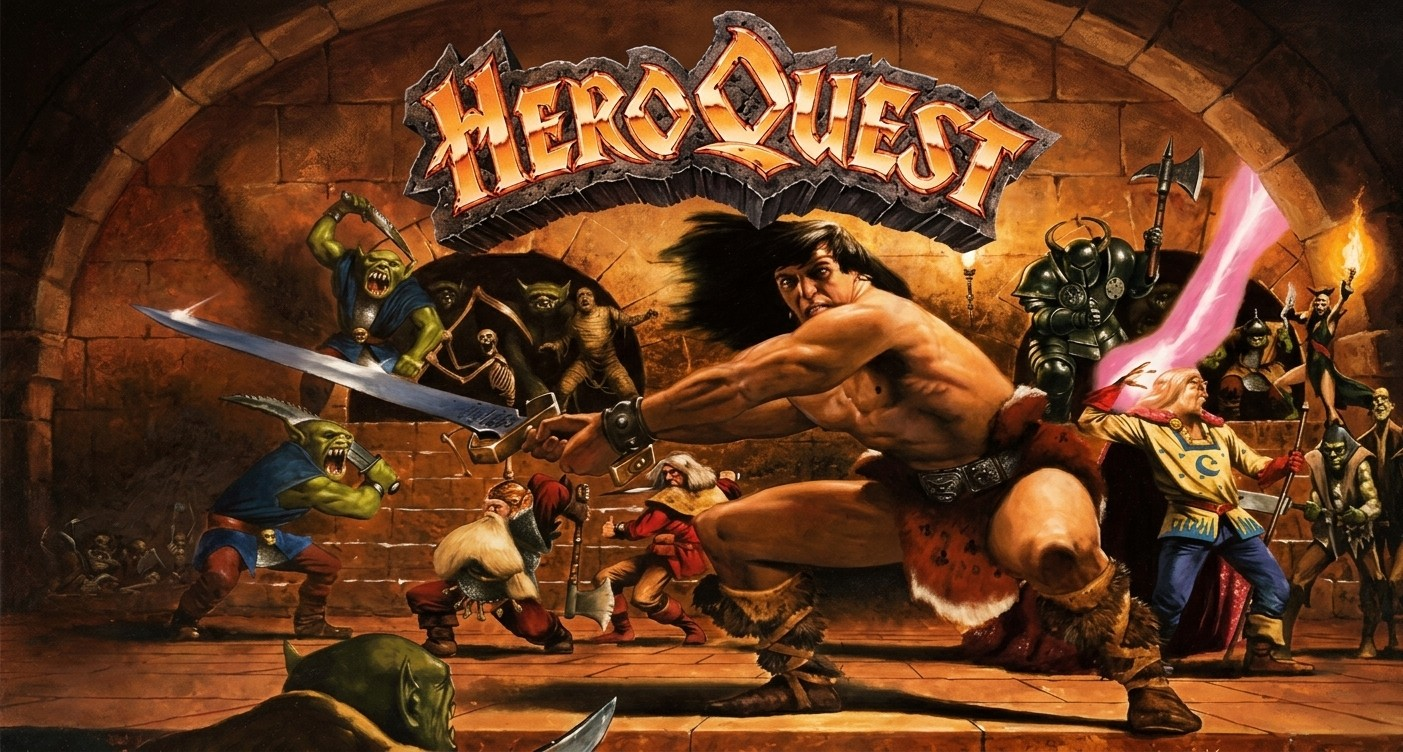
\includegraphics[width=1.6\paperwidth]{images/portada.jpg}}}%
\put(0.045\paperwidth,0.06\paperheight){
\includegraphics[width=0.30\paperwidth]{img/msx-logo.png}}}
\mbox{}\vfill
\begin{flushright}
\colorbox{ink}{\parbox{0.62\textwidth}{\raggedleft\color{white}\vspace{3pt}{\Huge\bfseries HEROQUEST}\\[6pt]{\Large\bfseries\tUserManual}\\[3pt]{\large\tPlatform{} \textperiodcentered{} \tVersion{} \versionjuego}\\[4pt]{\small\tCoverLine}\vspace{4pt}}}
\end{flushright}
\newpage
\thispagestyle{empty}
\begin{center}
\vspace*{1.2cm}
{\fontsize{34}{38}\selectfont\bfseries\textcolor{accent}{HEROQUEST}}\\[6pt]
{\Large\tPlatform}\\[1cm]

\includegraphics[height=2.2cm]{img/msx-logo.png}\\[1cm]
\tOriginal: \textbf{\originalPublisher}, \originalYear.\\[3pt]
\tPort: \textbf{\portAuthor}, \portYear.\\[3pt]
\tVersion{} \versionjuego\\[1cm]
\includegraphics[width=0.92\linewidth]{img/montage-\manlang.png}
\end{center}
\vfill
{\small\tHomage}
\newpage
\hypersetup{pageanchor=true}
\tableofcontents
\clearpage
\input{content-\manlang}
\clearpage
\input{credits-\manlang}
\input{label-\manlang}
\end{document}
"
\documentclass[a4paper,11pt]{article}
\providecommand{\manlang}{es}
\usepackage[utf8]{inputenc}
\usepackage[T1]{fontenc}
\usepackage{helvet}
\renewcommand{\familydefault}{\sfdefault}
% HeroQuest facts, shared by both editions.
\newcommand{\gameTitle}{HeroQuest}
\newcommand{\versionjuego}{1.0}
\newcommand{\originalPublisher}{Gremlin Graphics}
\newcommand{\originalYear}{1991}
\newcommand{\portAuthor}{DiHalt}
\newcommand{\portYear}{2026}
\newcommand{\accentRGB}{190,50,35}

\input{lang-\manlang}
\usepackage[margin=2.2cm,top=2.4cm,bottom=2.4cm]{geometry}
\usepackage{graphicx,xcolor,booktabs,tabularx,array,float,caption,fancyhdr,eso-pic,parskip,microtype}
\usepackage[hidelinks,pdftitle={HeroQuest \tPlatform{} -- \tManual{} v\versionjuego},pdfauthor={DiHalt}]{hyperref}
\graphicspath{{images/}{img/}}
\definecolor{accent}{RGB}{\accentRGB}
\definecolor{sangre}{RGB}{190,50,35}
\definecolor{pergamino}{RGB}{246,239,226}
\definecolor{ink}{RGB}{8,8,20}
\captionsetup{font=small,labelfont=bf}
\setlength{\parindent}{0pt}
\setlength{\headheight}{14pt}
\setcounter{secnumdepth}{2}
\setcounter{tocdepth}{2}
\setlength{\emergencystretch}{2em}
\raggedbottom
\pagestyle{fancy}\fancyhf{}
\fancyhead[L]{\small\textcolor{accent}{\textbf{HEROQUEST}} \tPlatform}
\fancyhead[R]{\small\tManual}
\fancyfoot[C]{\small\thepage}
\renewcommand{\headrulewidth}{0.4pt}
\newcommand{\chapter}[1]{\section{\textcolor{accent}{#1}}}
\newcommand{\key}[1]{{\fboxsep=2.5pt\fbox{\textbf{\strut #1}}}}
\newcommand{\pant}[1]{\textbf{#1}}
\newcommand{\pantalla}[3][0.78]{\begin{figure}[!htbp]\centering\includegraphics[width=#1\linewidth]{#2}\caption{#3}\end{figure}}
\newcommand{\dospantallas}[3]{\begin{figure}[!htbp]\centering\includegraphics[width=0.485\linewidth]{#1}\hfill\includegraphics[width=0.485\linewidth]{#2}\caption{#3}\end{figure}}
\newcommand{\aviso}[2]{\par\medskip\noindent\fcolorbox{accent}{pergamino}{\parbox{\dimexpr\linewidth-2\fboxsep-2\fboxrule\relax}{\textbf{\color{accent}#1}\par\smallskip #2}}\par\medskip}
\newcommand{\ficha}[4]{\par\medskip\noindent\begin{minipage}[t]{0.20\linewidth}\vspace{0pt}\centering\includegraphics[width=0.70\linewidth]{#1}\end{minipage}\hfill\begin{minipage}[t]{0.77\linewidth}\vspace{0pt}{\large\bfseries\color{accent}#2}\par\smallskip{\small #3}\par\smallskip #4\end{minipage}\par\medskip}
\newcommand{\aventura}[2]{\subsection*{\color{accent}#1.\ #2}\addcontentsline{toc}{subsection}{#1.\ #2}}
\newcommand{\objetivo}[1]{\par\smallskip\textbf{\tObjective} #1\par}
\newcommand{\consejos}[1]{\par\smallskip\textbf{\tTips} #1\par}
\newcolumntype{L}{>{\raggedright\arraybackslash}X}
\begin{document}
\hypersetup{pageanchor=false}
% Full-page cover, as in the Sol Negro reference.
\thispagestyle{empty}
% Frame the original landscape artwork at a smaller scale: the complete
% painted HEROQUEST title fits across the page, above the manual details.
\AddToShipoutPictureBG*{%
\put(0,0){\color{ink}\rule{\paperwidth}{\paperheight}}%
\put(0.5\paperwidth,\paperheight){\makebox(0,0)[t]{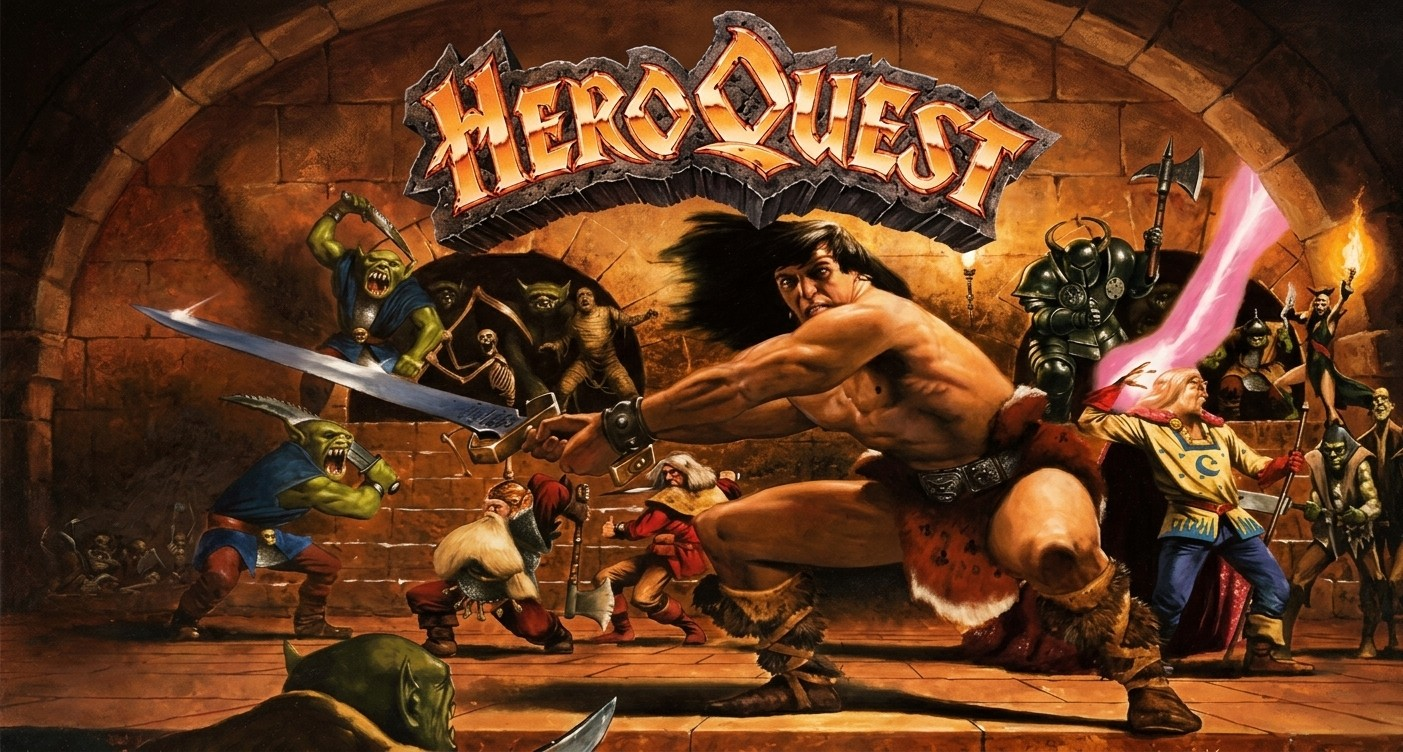
\includegraphics[width=1.6\paperwidth]{images/portada.jpg}}}%
\put(0.045\paperwidth,0.06\paperheight){
\includegraphics[width=0.30\paperwidth]{img/msx-logo.png}}}
\mbox{}\vfill
\begin{flushright}
\colorbox{ink}{\parbox{0.62\textwidth}{\raggedleft\color{white}\vspace{3pt}{\Huge\bfseries HEROQUEST}\\[6pt]{\Large\bfseries\tUserManual}\\[3pt]{\large\tPlatform{} \textperiodcentered{} \tVersion{} \versionjuego}\\[4pt]{\small\tCoverLine}\vspace{4pt}}}
\end{flushright}
\newpage
\thispagestyle{empty}
\begin{center}
\vspace*{1.2cm}
{\fontsize{34}{38}\selectfont\bfseries\textcolor{accent}{HEROQUEST}}\\[6pt]
{\Large\tPlatform}\\[1cm]

\includegraphics[height=2.2cm]{img/msx-logo.png}\\[1cm]
\tOriginal: \textbf{\originalPublisher}, \originalYear.\\[3pt]
\tPort: \textbf{\portAuthor}, \portYear.\\[3pt]
\tVersion{} \versionjuego\\[1cm]
\includegraphics[width=0.92\linewidth]{img/montage-\manlang.png}
\end{center}
\vfill
{\small\tHomage}
\newpage
\hypersetup{pageanchor=true}
\tableofcontents
\clearpage
\input{content-\manlang}
\clearpage
\input{credits-\manlang}
\input{label-\manlang}
\end{document}
